% This example is a LaTeX document showing how to use the lmproj class to
% write your report. The chapter headings are by no means prescriptive. Instead
% use an appropriate report structure for your project as you see fit.
% Use pdflatex and bibtex to process the file, creating a PDF file as output 
% (there is no need to use dvips when using pdflatex).

% Modified 

\documentclass{lmproj}
\usepackage{graphicx}
\graphicspath{ {images/} }




\begin{document}
\title{Bridging the gap between offline and online learning}
\author{Avgerinos Fotios \\
        Dunlop Fraser \\
        Constambeys Timotheos \\
        Zoulis Nickolas}
\date{18 December 2015}
\maketitle
\begin{abstract}

The abstract goes here

\end{abstract}
\educationalconsent
\tableofcontents
%==============================================================================
\chapter{Introduction}
\label{intro}

\section{Motivation}
\label{intro}

Over the last decade the area of data storage, manipulation and analysis has rapidly evolved as the previous techniques and infrastructures struggled to cope with the continuous data growth and demand rate. Algorithms and systems that used to perform well, could not handle the data explosion. Companies such as Yahoo and Google realized Moore's Law is not coming to their rescue anymore and started investing on research of developing systems that could scale linearly, instead of vertically, as data volume was increasing. 

The dawn of Big Data era was marked by the development of software infrastructures that could run on commodity hardware and exploit redundancy in order to provide availability and fault tolerance. Their workflow was targeting to partition the job to numerous physical nodes in order to decrease the total computation time. These systems can be characterized as (offline) batch processing, because they compute over batches of data and do not have the requirement to respond in realtime. Many such systems may require multiple chaining passes over the data in order to provide a result.

With the advancement to Web 2.0 and the rise of social networks as well as the notion of the Internet of Things (machines equipped with sensors, transferring data at an arbitrary rate) altered the existing game rules. The need was for quick response to incoming data, without having to keep track of them or perform any asynchronous analysis over them. That said, many systems started to appear that could handle the input streaming and perform online, instead of offline learning techniques. 

\section{Problem Definition}
\label{intro}

A lot of research on both offline and online systems has been made over the last years, resulting to the recording of successful commercial usage in numerous use cases. Individually speaking, batch systems can provide offline query computation, whereas streaming systems can provide online query computation. The first ones may take a lot of time to respond, but they take into account the whole picture and can recover in case of corrupted or noisy data without losing any information, as they could simply restart computations. The latter ones, while can provide low latency answers in realtime, follow the trend of input data, which is desirable if this is the use case, if any errors occur, they cannot just simply restart without losing information from their latest safepoint to the time the error spotted.

So what if we wanted a robust system that could provide answers as soon as possible and an always-on experience, without compromising quality? A need for a hybrid emerges, and it was Nathan Marz who first came up with the term Lambda Architecture, which describes an architecture resilient to faults, while still remaining highly available from the perspective of a client. Lambda Architecture is comprised of three basic components, the Batch, the Speed and the Serving layers. Batch layer is responsible for computing query views asynchronously over batch of data. Stream is responsible for handling the most recent data input to the system and provide answers on-the-fly by maintaining an online learning model. Last but not least, the Serving layer is responsible for indexing the views of both the other layers so they can be queried in a low latency, ad-hoc way.

The problem that arises is how the views of Batch and Stream can be merged and in what way. Who should be trusted more, what kind of methods should be used for the aggregation and how applicable would one method be in a different use case scenario are only some of the research questions that naturally arise. 

\section{Contributions}
\label{intro}

Out contribution is to investigate the trade-offs of low latency responses over quality when applying machine learning algorithms over Lambda Architecture. We implemented a proof-of-concept system that follows this design and experimented with a well-known unsupervised learning clustering algorithm, K-Means. 


%==============================================================================
\chapter{Related Work}
\label{relatedwork}

\section{Theoritical Background on K-Means}
\label{relatedwork}

\section{Batch Processing}
\label{relatedwork}

\section{Stream Processing}
\label{relatedwork}

\section{Lambda Architecture}
\label{relatedwork}


%==============================================================================
\chapter{Our system - Thunderstorm}
\label{systemdescr}

\section{Overall Design}
\label{systemdescr}

For our project's purposes we have chosen to use the below systems for each component of Lambda Architecture:

\begin{itemize}
	\item Serving layer with Apache HBase
	\item Batch layer with Apache Spark
	\item Stream layer with Apache Storm
\end{itemize}

\begin{figure}[h]
\centering
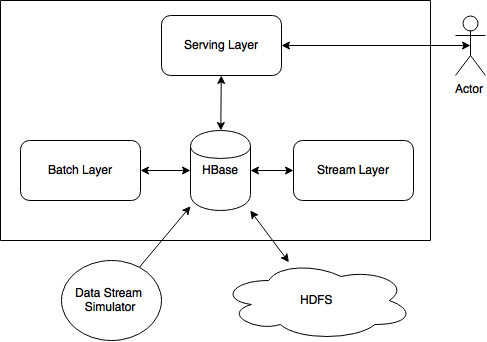
\includegraphics[width=10cm, height=8cm]{system}
\caption{An abstract picture of how our system is formulated}
\end{figure}


\section{Serving Layer}
\label{systemdescr}

\section{Batch Layer}
\label{systemdescr}

\section{Streaming Layer}
\label{systemdescr}

\section{Interface between the layers}
\label{systemdescr}




%==============================================================================
\chapter{Offline/Online K-Means}
\label{kmeans}

\section{Theoritical Solution outline}
\label{kmeans}

\section{Baseline Solution}
\label{kmeans}

\section{Fusion Scheme}
\label{kmeans}

\section{Hybrids}
\label{kmeans}



%==============================================================================
\chapter{Evaluation}
\label{evaluation}

\section{Setup}
\label{evaluation}

\section{Results}
\label{evaluation}

\section{Discussion}
\label{evaluation}


%==============================================================================
\section{Conclusions}
\label{conclusions}


%==============================================================================
\bibliographystyle{plain}
\bibliography{example}
\end{document}
